\documentclass{article}

\usepackage[submission]{colm2026_conference}
\usepackage{booktabs}
\usepackage{microtype}
\usepackage{hyperref}
\usepackage{enumitem}
\usepackage{xcolor}
\usepackage{graphicx}
\usepackage{url}
\usepackage{tikz}
\usepackage{pgfplots}
\usepackage{amsmath}
\usepackage{lineno}
\pgfplotsset{compat=1.18}

\definecolor{darkblue}{rgb}{0, 0, 0.5}
\hypersetup{
  colorlinks=true,
  linkcolor=darkblue,
  citecolor=darkblue,
  urlcolor=darkblue
}

\newcommand{\method}{Critical Span Guard}
\newcommand{\tcfr}{TCFR}

\title{Do Not Anonymize Away the Answer:\
Measuring Task-Critical Meaning Loss in Text De-identification}

\author{Anonymous Authors}
\date{}

\begin{document}

\ifcolmsubmission
\linenumbers
\fi

\maketitle

\begin{abstract}
Text de-identification is often evaluated as a span removal problem: did a
system remove names, dates, locations, contact information, and other explicit
identifiers?  For sensitive text used in foundation-model workflows, this is
necessary but incomplete.  A transformed clinical vignette or legal case
excerpt can pass a privacy-oriented screen while removing the medication dose,
lab value, statutory article, procedural posture, or legal claim needed for
downstream reasoning.  We study this failure mode through a small
clinical/legal benchmark for utility-preserving anonymization.  The benchmark
pairs privacy labels with task-critical facts and downstream QA items.  We
introduce \textit{Task-Critical Fact Retention} (\tcfr), a fact-level utility
metric, and \method, a low-cost protocol that extracts privacy spans and
important domain facts, anonymizes under preservation constraints, verifies the
result, and applies a deterministic safety/repair layer.  In a 150-example
non-oracle LLM run, \method{} achieves zero measured direct identifier leaks,
lower quasi-identifier risk (0.13 versus 1.73 for generic prompting and 0.57
for privacy-first prompting), and higher audited task-critical fact retention
(0.99 versus 0.94 and 0.53).  A handwritten stress slice further shows why
the problem is not reducible to ``redact more'': some sensitive facts, such as
pregnancy, sexual orientation, domestic violence, or minority status, can also
be the task-critical answer.  The results support evaluating de-identification
systems by both privacy protection and retained domain meaning.
\end{abstract}

\section{Introduction}

Sensitive clinical and legal text is valuable for retrieval-augmented
generation, supervised fine-tuning, model evaluation, safety auditing, and
synthetic-data generation.  The usual first step before such use is
de-identification, anonymization, or pseudonymization.  However, a system
optimized only for removing personally identifying information can destroy the
very facts that make the text useful.  In a clinical note, replacing
``methotrexate 15 mg weekly'' with ``a medication'' may preserve broad topical
similarity while breaking the answer to a treatment question.  In a legal
excerpt, replacing ``Article 6'' with ``a specified article'' removes the legal
basis needed to reason about the claim.  These are not cosmetic changes: they
alter the information that downstream models or evaluators are expected to use.

This tension is especially important for foundation-model data pipelines.  A
release pipeline that over-redacts data may be privacy-conservative but unable
to support clinical decision-support evaluation, legal QA, or domain-specific
retrieval.  A pipeline that preserves all clinically or legally meaningful
facts may leave quasi-identifiers, rare events, or sensitive attributes that can
aid re-identification.  In practice, data stewards must make policy choices
about which facts are safe to preserve, which facts must be generalized, and
which facts are too sensitive to release even when they are task-relevant.  Yet
many evaluations still reduce de-identification to span-level recall over
predefined identifier categories.

We ask a practical question: \emph{after anonymization, is the
transformed text still useful for the domain task it was meant to support?}  We
focus on two domains where the privacy--utility tension is concrete.
Clinical-style vignettes contain diagnoses, medications, doses, labs, symptoms,
procedures, and timelines.  Public legal snippets derived from the Text
Anonymization Benchmark (TAB) contain application identifiers, party roles,
claims, legal articles, procedural facts, confidential attributes, and outcomes
\cite{pilan2022tab}.  Existing tools such as Microsoft Presidio \cite{presidio}
and regulatory frameworks such as HIPAA de-identification guidance
\cite{hhsdeid} are essential privacy infrastructure, but they do not by
themselves answer whether the remaining text preserves task-critical meaning.

This paper makes four contributions:
\begin{itemize}[leftmargin=*,nosep]
\item We construct a 150-example controlled benchmark with synthetic clinical
vignettes and TAB-derived legal snippets, each annotated with direct
identifiers, quasi-identifiers, task-critical facts, and downstream QA items.
\item We propose \textit{Task-Critical Fact Retention} (\tcfr), a fact-level
utility metric that distinguishes retained domain meaning from generic surface
similarity.
\item We introduce \method, a simple anonymization protocol that extracts
privacy spans and task-critical facts, anonymizes under explicit preservation
constraints, and applies deterministic safety/repair rules for direct
identifiers and known domain-specific failure modes.
\item We provide a bounded empirical audit showing that generic prompting tends
to preserve utility but leak identifiers, privacy-first prompting removes
identifiers but often removes the answer, and task-aware structure improves the
observed privacy--utility frontier.
\end{itemize}

We argue that span-level privacy evaluation alone
can both miss residual risk and reward over-redaction.  For sensitive text used
in foundation-model workflows, a more useful evaluation must ask two questions
jointly: what identifying information remains, and what domain meaning has been
lost?

\section{Related Work}

\paragraph{Text de-identification.}
Clinical de-identification has a long history in shared tasks and patient-note
benchmarks.  Early neural systems framed the problem as sequence labeling over
protected-health-information spans \cite{dernoncourt2016patientnotes}, while
annotation resources from i2b2 and related challenges supported systematic PHI
recognition and normalization \cite{stubbs2015automated}.  Recent work has
explored stronger neural and LLM-based de-identification, but the dominant
evaluation mode is still identifier detection or span replacement.  This is a
necessary component of privacy evaluation, but it does not directly measure
whether clinically material facts such as drugs, doses, lab values, and
procedures remain intact.

\paragraph{Legal anonymization.}
TAB provides an important benchmark for legal-text anonymization by annotating
European Court of Human Rights cases with entity spans, masking decisions,
confidential attributes, and coreference relations \cite{pilan2022tab}.  Later
work on neural legal anonymization further shows that legal documents require
more than generic named-entity recognition because case identifiers, party
roles, procedural details, and confidential attributes interact with legal
meaning \cite{papadopoulou2023neural}.  Our legal split builds on TAB but adds a
utility target: legal article references, claims, outcomes, and procedural
facts should be preserved when they are necessary for downstream reasoning.

\paragraph{Privacy risk beyond direct identifiers.}
Classical privacy work distinguishes direct identifiers from quasi-identifiers:
attributes that may not identify a person alone but can do so in combination
\cite{sweeney2002kanonymity,narayanan2008robust}.  Differential privacy gives a
formal framework for aggregate releases and learning algorithms
\cite{dwork2006calibrating}, but most practical text anonymization pipelines do
not provide such guarantees.  Recent LLM privacy work shows that powerful
models can infer personal attributes from seemingly innocuous text
\cite{staab2023beyond}.  Recent anonymization benchmarks therefore increasingly
consider residual re-identification risk and utility together
\cite{loiseau2025taueval,krco2026ratbench}, and contemporaneous adaptive
anonymization work treats the privacy--utility tradeoff as a task-specific
prompt-optimization problem \cite{loiseau2026adaptive}.  We share this
motivation, but make the utility target explicit at the level of domain facts
and QA answers.

\paragraph{Utility and faithfulness metrics.}
Generic text-generation metrics such as token overlap, embedding similarity, or
BERTScore \cite{bertscore} can be useful diagnostics, but they do not encode
what domain facts must be preserved.  High similarity to the original can even
be a warning sign in anonymization because identifiers and quasi-identifiers
may remain.  Conversely, low similarity may be acceptable if the transformed
text preserves the clinically or legally relevant answer.  This motivates a
fact-level metric rather than relying only on surface similarity.

\section{Benchmark and Task}

\paragraph{Task definition.}
Given an input text $x$, a de-identification method outputs transformed text
$\hat{x}$.  Each example contains three types of annotation: direct identifiers
$D$, quasi-identifiers $Q$, and task-critical facts $F$.  Direct identifiers
include names, contact information, exact dates, medical record numbers, legal
application numbers, and named institutions tied to a person.  Quasi-identifiers
include age, occupation, city, nationality, sensitive attributes, family
relations, rare events, and combinations of details that may enable linkage.
Task-critical facts include information needed to answer a domain question:
clinical diagnoses, labs, medications, doses, symptoms, procedures, timelines,
or legal articles, claims, procedures, outcomes, and reasoning.  A good output
should remove or generalize $D$ and high-risk $Q$ while preserving the facts in
$F$ at the specificity required by the downstream task.

\paragraph{Clinical split.}
We generate 75 synthetic clinical vignettes from templates.  Each example
contains direct identifiers such as patient name, clinician name, clinic, date,
medical record number, phone number, and email; quasi-identifiers such as age,
city, and occupation; and task-critical facts such as diagnosis, medication,
dose, lab result, symptom duration, imaging result, or treatment plan.  The
clinical split is synthetic by design: it provides controlled utility labels
without exposing real protected health information.  It should be interpreted
as a controlled stress test, not as evidence of performance on real clinical
notes.

\paragraph{Legal split.}
We sample 75 short excerpts from TAB, an open-source corpus of English-language
European Court of Human Rights cases annotated with personal identifiers,
masking decisions, confidential attributes, and coreference relations
\cite{pilan2022tab}.  For each sampled snippet, we keep short procedure,
complaint, and outcome sentences when available.  We use TAB spans for privacy
labels and heuristic extraction plus manual spot checks for legal articles,
claims, outcomes, and QA answers.  This lets us study legal meaning without
processing private legal files.

\paragraph{Stress slice.}
We also construct a 12-example handwritten diagnostic slice that stresses cases
where privacy and utility overlap: pregnancy, sexual orientation, domestic
violence, Roma marriage, exact ages, rare occupations, case labels, secret
evidence, exact legal article/protocol specificity, numeric labs, and dose
preservation.

\section{Metrics}

We report privacy and utility metrics together.  \textit{Direct leak} is the
fraction of rows where any gold direct identifier remains in the anonymized
text.  \textit{QI risk} is the mean quasi-identifier risk score, where retained
specific dates, locations, occupations, sensitive attributes, or combinations of
details increase the risk.  We also report direct, quasi, and all-span privacy
recall: the fraction of gold privacy spans not found verbatim after
anonymization.

For utility, exact \tcfr{} measures the fraction of gold task-critical facts
retained by deterministic phrase or alias matching:
\begin{equation}
\mathrm{TCFR}(\hat{x}) = \frac{1}{|F|}\sum_{f \in F} \mathbb{1}[f \text{ is retained in } \hat{x}].
\end{equation}
Exact matching is reproducible but conservative because faithful paraphrases
may not match the gold string.  We therefore also report audited \tcfr{} using a
structured LLM fact judge that marks each fact as preserved,
generalized-but-acceptable, omitted, contradicted, or unclear.  The judge is
strict for medication names, doses, lab values, legal Article numbers, outcomes,
and legal claims.  \textit{QA consistency} asks whether downstream questions can
still recover the gold answers from the anonymized text.  Finally, we report
surface metrics such as token F1, TF-IDF cosine, and edit rate only as
diagnostic foils, not as privacy or task-utility guarantees.

\section{Methods}

We compare three non-oracle LLM anonymizers in the 150-example run.  All
methods operate on the same inputs and are evaluated with the same gold privacy
and utility annotations.

\paragraph{Generic LLM.}
The generic prompt asks the model to remove personally identifying information
while preserving document meaning.  It resembles the simple instruction a data
steward might give to a general-purpose model.  This baseline tests whether
broad de-identification instructions are sufficient.

\paragraph{Privacy-first LLM.}
The privacy-first prompt asks the model to remove or generalize any information
that could identify a person, including rare locations, exact dates, named
institutions, rare occupations, unique events, and combinations of details.  It
is intentionally conservative.  This baseline tests the cost of resolving
uncertainty by redacting or generalizing aggressively.

\paragraph{\method.}
\method{} adds structure.  First, an
extraction prompt identifies privacy spans and task-critical domain facts.
Second, an anonymization prompt receives these structures and is instructed to
replace direct identifiers with typed placeholders, generalize
quasi-identifiers when possible, preserve task-critical facts, and use the least
identifying version of facts that are both privacy-relevant and task-critical.
For clinical text, the prompt explicitly protects medications, doses, labs,
diagnoses, symptoms, imaging findings, and meaningful timelines.  For legal
text, it protects legal article/statute numbers, claims, procedural posture,
outcomes, and reasoning, while treating legal case/application numbers as direct
identifiers.  Third, a verification/repair prompt checks for leaked direct
identifiers, generalizable quasi-identifiers, omitted facts, contradictions, and
invented facts.  Finally, a deterministic safety/repair layer replaces direct
identifiers such as case/application numbers, dates, MRNs, phone numbers,
emails, names, and institutions, and repairs known domain mistakes such as legal
Article over-generalization and medication placeholdering.

\paragraph{Diagnostic local baselines.}
We also run local diagnostic baselines on the original benchmark, a 200-example
local expansion, and the stress slice: regex rules, Presidio, direct-span oracle
replacement, privacy-first oracle redaction, and a CSG oracle using gold
benchmark annotations.  These oracle variants are not deployable systems; they
diagnose upper bounds and failure modes.

\section{Experimental Setup}

The promoted non-oracle run contains 150 examples: 75 synthetic clinical
vignettes and 75 TAB-derived legal snippets.  The LLM methods are run with a
GPT model.  The exact model is not central to
our claim: the paper evaluates prompt protocols and safety layers under a
bounded budget rather than training a new model.  We use no real protected
health information.  Clinical examples are synthetic, and legal examples are
public TAB-derived snippets.

We compute deterministic privacy and exact-utility metrics from gold spans and
facts.  We then run an LLM-assisted fact-retention audit over the anonymized
outputs.  Paired deltas are computed over the same examples to compare
\method{} against each baseline.  We also inspect
qualitative failures and maintain explicit claim boundaries: the privacy metrics
are string/span and heuristic risk audits, not k-anonymity, differential
privacy, legal compliance, or protection against an adversary with external
databases.

\section{Results}

\begin{table}[t]
\centering
\small
\begin{tabular}{lccccc}
\toprule
Method & Direct leak $\downarrow$ & QI risk $\downarrow$ & Exact \tcfr{} $\uparrow$ & Audited \tcfr{} $\uparrow$ & QA $\uparrow$ \\
\midrule
Generic LLM & 0.18 & 1.73 & 0.81 & 0.94 & 0.89 \\
Privacy-first LLM & 0.00 & 0.57 & 0.40 & 0.53 & 0.41 \\
\method{} & 0.00 & 0.13 & 0.88 & 0.99 & 0.97 \\
\bottomrule
\end{tabular}
\caption{Main 150-example non-oracle results.  Generic prompting preserves many facts but leaks identifiers; privacy-first prompting protects direct identifiers but often removes the answer; \method{} improves the measured privacy--utility frontier.}
\label{tab:main}
\end{table}

Table~\ref{tab:main} shows the core privacy--utility tradeoff.  Generic
prompting preserves many task facts, but leaks direct identifiers in 27 of 150
examples and has high QI risk.  Privacy-first prompting removes all measured
direct identifiers, but exact \tcfr{} falls to 0.40 and QA consistency to
0.41.  \method{} achieves zero measured direct leaks, the lowest overall QI
risk, audited \tcfr{} of 0.99, and QA consistency of 0.97.

\begin{table}[t]
\centering
\small
\begin{tabular}{llccccc}
\toprule
Domain & Method & Direct leak & QI risk & Exact \tcfr{} & Audited \tcfr{} & QA \\
\midrule
Clinical & Generic & 0.03 & 2.03 & 0.70 & 0.93 & 0.85 \\
Clinical & Privacy-first & 0.00 & 1.07 & 0.19 & 0.46 & 0.23 \\
Clinical & \method{} & 0.00 & 0.00 & 0.82 & 1.00 & 1.00 \\
\midrule
Legal & Generic & 0.33 & 1.44 & 0.92 & 0.94 & 0.92 \\
Legal & Privacy-first & 0.00 & 0.08 & 0.60 & 0.60 & 0.60 \\
Legal & \method{} & 0.00 & 0.25 & 0.95 & 0.99 & 0.95 \\
\bottomrule
\end{tabular}
\caption{Domain split for the 150-example non-oracle run.  The legal split exposes the hardest residual tradeoff: privacy-first redaction attains lower QI risk by deleting or generalizing legally meaningful details, while \method{} preserves more legal utility but retains a small number of task-overlapping quasi-identifiers.}
\label{tab:domain}
\end{table}

The domain split in Table~\ref{tab:domain} reveals different failure modes.
In clinical examples, generic prompting leaves nearly all quasi-identifiers,
whereas privacy-first prompting often replaces specific diagnoses, drugs, labs,
or doses with vague placeholders.  \method{} removes all measured clinical QI
hits while retaining almost all audited facts.  In legal examples, the frontier
is harder.  Privacy-first prompting has lower QI risk than \method{} on the
legal subset because it generalizes legal claims, jurisdictions, statutes, or
sensitive attributes.  This improves the measured privacy score but damages the
legal utility target.

The span-level privacy audit agrees with the row-level picture.  \method{}
reaches direct span recall of 1.00 and all privacy-span recall of 0.98,
compared with 0.92 and 0.77 for generic prompting and 1.00 and 0.96 for
privacy-first prompting.  Paired deltas on the same examples sharpen this
interpretation.  Relative to generic prompting, \method{} reduces direct-leak
rate by 0.18 and QI risk by 1.61; on legal rows alone, the QI reduction is
1.19.  Relative to privacy-first prompting, it improves exact \tcfr{} by 0.49,
audited \tcfr{} by 0.47, and QA consistency by 0.56.  The domain-level
audited-\tcfr{} gains over privacy-first are 0.54 on clinical rows and 0.39 on
legal rows.  The legal-only QI comparison is an
important caveat: \method{} is slightly worse than privacy-first prompting on
legal QI risk because it intentionally preserves some legal facts that overlap
with quasi-identifying content.

As a sample-size diagnostic, we also ran a bounded 300-example diagnostic
expansion, adding 75 clinical and 75 legal rows beyond the promoted n150 run.
The qualitative frontier persists: \method{} has zero measured direct leaks, QI
risk 0.21, and audited \tcfr{} 0.99, compared with 0.19, 1.79, and 0.93
for generic prompting and 0.00, 0.62, and 0.52 for privacy-first prompting.
On the added n200-to-n300 100-example slice alone, \method{} has zero direct
leak rows, 14 QI-hit rows, and audited \tcfr{} 0.99.  We keep n150 as the
promoted headline because the manuscript tables and completed manual-audit plan
remain anchored there; the n300 downstream bundle is synchronized but its
second-annotator packet has not yet been completed.  Thus n300 is sample-size
robustness evidence, not a promoted headline replacement.

To test judge dependence, we also ran an external GPT-5.5 fact-retention audit
over all promoted n150 outputs.  The stronger judge is stricter than the
low-cost judge but preserves the utility ordering: audited \tcfr{} is
0.92 for \method{}, 0.90 for generic prompting, and 0.41 for privacy-first
prompting.  The paired \method{}-minus-generic audited-\tcfr{} gain is small and
statistically uncertain (0.02), while the same rows still show generic direct
leakage (0.18) and QI risk (1.73) versus zero direct leakage and QI risk 0.13
for \method{}.  Fact-label agreement with the
original audit is 0.92, 0.95, and 0.83 respectively, with most disagreements
caused by strict clinical numeric or legal specificity.  A GPT-5.5 adversarial
privacy audit on the 20 hardest rows is similarly conservative:
generic prompting has direct
privacy flags on 60\% of rows, \method{} on 5\%, and privacy-first prompting on
0\%, but privacy-first is the same method that loses most task-critical facts.
We treat these external audits as robustness checks, not as expert annotation.
Table~\ref{tab:followup} combines the follow-up checks used for claim
triangulation.  The bounded n30 GPT-5.5 anonymization screen shows that stronger
generic prompting can remove obvious direct leaks on selected stress cases, but
privacy-first prompting still loses utility and \method{} remains the best
audited-\tcfr{} corner.  \method{} does not have the lowest upgraded QI risk on
that stress screen, so we treat the result as reviewer-risk triage rather than
a model-scaling claim.

\begin{table}[t]
\centering
\small
\resizebox{\linewidth}{!}{%
\begin{tabular}{lcccccc}
\toprule
Method & n150 audit & GPT-5.5 fact60 & Full-n150 & Hard20 severe & Fixed30 audit & GPT-5.5 anon n30 \\
\midrule
Generic LLM & 0.94 & 0.87 & 0.90 & 1.00 & 0.84 & 0.81 \\
Privacy-first LLM & 0.53 & 0.48 & 0.41 & 0.70 & 0.51 & 0.42 \\
\method{} & 0.99 & 0.92 & 0.92 & 0.90 & 0.97 & 0.89 \\
\bottomrule
\end{tabular}%
}
\caption{Follow-up robustness checks.  Columns report audited \tcfr{} except Hard20 severe, which is the GPT-5.5 adversarial privacy severe-flag rate on the 20 hardest rows.  Full-n150 is completed model-auditor coverage for the promoted n150 outputs, but is not expert/human annotation.  Fixed30 is a deliberately hard manual-style subset; GPT-5.5 anon n30 is a bounded stronger-model screen, not a broad model-scaling result.}
\label{tab:followup}
\end{table}


Figure~\ref{fig:frontier} summarizes the main privacy--utility frontier: the
task-aware protocol moves toward lower QI risk without collapsing audited
fact retention.

% Auto-generated by src/make_paper_figures.py; do not edit by hand.
\begin{figure}[t]
\centering
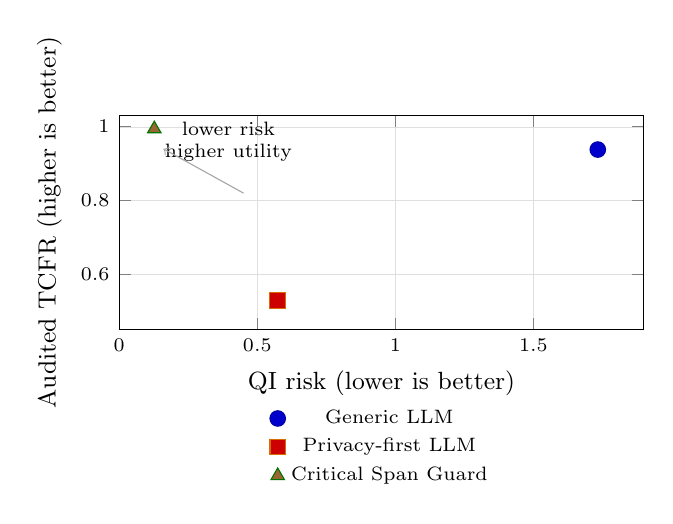
\begin{tikzpicture}
\begin{axis}[
  width=0.68\linewidth,
  height=4.3cm,
  xmin=0,
  xmax=1.90,
  ymin=0.45,
  ymax=1.03,
  xlabel={QI risk (lower is better)},
  ylabel={Audited \tcfr{} (higher is better)},
  grid=both,
  grid style={line width=.1pt, draw=gray!25},
  tick label style={font=\scriptsize},
  label style={font=\small},
  legend style={font=\scriptsize, draw=none, fill=none, at={(0.5,-0.32)}, anchor=north, legend columns=1},
  clip=false,
]
\addplot+[only marks, mark=*, mark size=2.8pt, color=blue!65!black] coordinates {(1.733,0.938)};
\addlegendentry{Generic LLM}
\addplot+[only marks, mark=square*, mark size=2.8pt, color=orange!85!black] coordinates {(0.573,0.529)};
\addlegendentry{Privacy-first LLM}
\addplot+[only marks, mark=triangle*, mark size=2.8pt, color=green!45!black] coordinates {(0.127,0.994)};
\addlegendentry{Critical Span Guard}
\node[font=\scriptsize, align=center, anchor=west] at (axis cs:0.13,0.96) {lower risk\\higher utility};
\draw[->, gray!70] (axis cs:0.45,0.82) -- (axis cs:0.16,0.94);
\end{axis}
\end{tikzpicture}
\caption{Privacy--utility frontier for the 150-example non-oracle LLM run. \method{} is closest to the upper-left target region: lower measured quasi-identifier risk and higher audited task-critical fact retention.}
\label{fig:frontier}
\end{figure}


\begin{table}[t]
\centering
\small
\begin{tabular}{lcccc}
\toprule
Stage & Direct leak & QI risk & Exact \tcfr{} & QA \\
\midrule
CSG draft & 0.07 & 1.03 & 0.88 & 0.97 \\
CSG verified & 0.07 & 1.03 & 0.88 & 0.97 \\
CSG + safety/repair & 0.00 & 0.13 & 0.88 & 0.97 \\
\bottomrule
\end{tabular}
\caption{\method{} ablation.  The verification prompt did not change deterministic metrics in this sample; the measured gain comes from the deterministic safety/repair layer.}
\label{tab:ablation}
\end{table}

Table~\ref{tab:ablation} is important for claim discipline.  In this
sample, the verification/repair prompt did not change deterministic metrics:
the draft and verified rows are numerically identical.  The measured gain comes
from the deterministic safety/repair layer, which closes eleven direct leaks,
reduces QI-risk rows from 74 to 11, repairs legal Article specificity losses,
and leaves eleven legal residual cases.  This result suggests that
LLM-generated anonymization should be paired with explicit deterministic checks,
not trusted as a single-pass transformation.

\begin{table}[t]
\centering
\small
\begin{tabular}{lccccc}
\toprule
Method & Token F1 & TF-IDF & Edit rate & Audited fact-fail rate & Privacy-fail rate \\
\midrule
Generic LLM & 0.78 & 0.71 & 0.25 & 0.24 & 0.75 \\
Privacy-first LLM & 0.58 & 0.47 & 0.46 & 0.79 & 0.27 \\
\method{} & 0.77 & 0.62 & 0.27 & 0.02 & 0.03 \\
\bottomrule
\end{tabular}
\caption{Surface similarity metrics are not sufficient proxies for privacy-safe utility.}
\label{tab:surface}
\end{table}

Table~\ref{tab:surface} addresses whether generic utility metrics are enough.
Generic prompting and \method{} have nearly identical token F1 against the
original text, and generic prompting has higher TF-IDF cosine similarity, but it
also has far higher privacy failure and audited fact failure rates.  Among the
225 method-example rows at or above the median TF-IDF cosine score, 73 still
have privacy failures and 34 still have audited fact loss.  Surface similarity
therefore rewards text that may be too close to the original and misses
task-critical failures; this is consistent with broader concerns that generic
text-generation metrics do not encode domain-specific faithfulness by
themselves \cite{bertscore}.

% Auto-generated by src/make_surface_failure_scatter.py; do not edit by hand.
\begin{figure}[t]
\centering
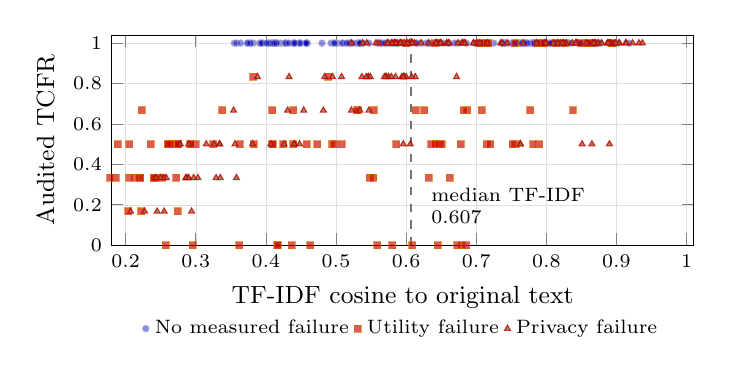
\begin{tikzpicture}
\begin{axis}[
  width=0.74\linewidth,
  height=4.25cm,
  xmin=0.18,
  xmax=1.01,
  ymin=0.00,
  ymax=1.04,
  xlabel={TF-IDF cosine to original text},
  ylabel={Audited \tcfr{}},
  grid=both,
  grid style={line width=.1pt, draw=gray!25},
  tick label style={font=\scriptsize},
  label style={font=\small},
  legend style={font=\scriptsize, draw=none, fill=none, at={(0.5,-0.30)}, anchor=north, legend columns=3},
  clip=false,
]
\addplot+[only marks, mark=*, mark size=1.25pt, color=gray!55, opacity=0.45] coordinates {(0.382,1.000) (0.396,1.000) (0.647,1.000) (0.502,1.000) (0.606,1.000) (0.615,1.000) (0.414,1.000) (0.588,1.000) (0.458,1.000) (0.531,1.000) (0.440,1.000) (0.404,1.000) (0.493,1.000) (0.538,1.000) (0.530,1.000) (0.565,1.000) (0.391,1.000) (0.518,1.000) (0.583,1.000) (0.374,1.000) (0.410,1.000) (0.355,1.000) (0.449,1.000) (0.421,1.000) (0.447,1.000) (0.378,1.000) (0.429,1.000) (0.439,1.000) (0.427,1.000) (0.441,1.000) (0.510,1.000) (0.458,1.000) (0.459,1.000) (0.538,1.000) (0.480,1.000) (0.596,1.000) (0.587,1.000) (0.429,1.000) (0.497,1.000) (0.577,1.000) (0.458,1.000) (0.634,1.000) (0.457,1.000) (0.378,1.000) (0.587,1.000) (0.415,1.000) (0.374,1.000) (0.416,1.000) (0.573,1.000) (0.403,1.000) (0.410,1.000) (0.521,1.000) (0.409,1.000) (0.393,1.000) (0.406,1.000) (0.559,1.000) (0.564,1.000) (0.566,1.000) (0.519,1.000) (0.524,1.000) (0.433,1.000) (0.394,1.000) (0.358,1.000) (0.415,1.000) (0.449,1.000) (0.509,1.000) (0.570,1.000) (0.441,1.000) (0.602,1.000) (0.547,1.000) (0.534,1.000) (0.498,1.000) (0.412,1.000) (0.756,1.000) (0.629,1.000) (0.622,1.000) (0.364,1.000) (0.830,1.000) (0.873,1.000) (0.781,1.000) (0.810,1.000) (0.867,1.000) (0.874,1.000) (0.814,1.000) (0.790,1.000) (0.674,1.000) (0.868,1.000) (0.902,1.000) (0.712,1.000) (0.846,1.000) (0.868,1.000) (0.781,1.000) (0.401,1.000) (0.850,1.000) (0.799,1.000) (0.715,1.000) (0.581,1.000) (0.763,1.000) (0.757,1.000) (0.769,1.000) (0.837,1.000) (0.833,1.000) (0.785,1.000) (0.776,1.000) (0.716,1.000) (0.742,1.000) (0.763,1.000) (0.653,1.000) (0.713,1.000) (0.701,1.000) (0.877,1.000) (0.891,1.000) (0.698,1.000) (0.771,1.000) (0.759,1.000) (0.781,1.000) (0.825,1.000) (0.826,1.000) (0.848,1.000) (0.615,1.000) (0.515,1.000) (0.535,1.000) (0.769,1.000) (0.703,1.000) (0.767,1.000) (0.818,1.000) (0.741,1.000) (0.780,1.000) (0.700,1.000) (0.785,1.000) (0.766,1.000) (0.787,1.000) (0.715,1.000) (0.896,1.000) (0.889,1.000) (0.867,1.000) (0.813,1.000) (0.792,1.000) (0.780,1.000) (0.533,1.000) (0.754,1.000) (0.712,1.000) (0.772,1.000) (0.795,1.000) (0.738,1.000) (0.773,1.000) (0.717,1.000) (0.660,1.000) (0.704,1.000) (0.714,1.000) (0.725,1.000) (0.805,1.000) (0.863,1.000) (0.868,1.000) (0.704,1.000) (0.740,1.000) (0.765,1.000) (0.739,1.000) (0.868,1.000) (0.811,1.000) (0.737,1.000) (0.700,1.000) (0.918,1.000) (0.718,1.000) (0.857,1.000) (0.821,1.000) (0.789,1.000) (0.859,1.000) (0.783,1.000) (0.783,1.000) (0.806,1.000) (0.737,1.000) (0.603,1.000) (0.808,1.000) (0.632,1.000) (0.712,1.000) (0.769,1.000) (0.746,1.000) (0.661,1.000) (0.710,1.000) (0.718,1.000) (0.534,1.000) (0.686,1.000) (0.669,1.000) (0.806,1.000) (0.710,1.000) (0.824,1.000)};
\addlegendentry{No measured failure}
\addplot+[only marks, mark=square*, mark size=1.25pt, color=orange!85!black, opacity=0.65] coordinates {(0.300,0.500) (0.267,0.500) (0.205,0.500) (0.273,0.500) (0.409,0.667) (0.338,0.667) (0.274,0.167) (0.221,0.333) (0.292,0.500) (0.221,0.333) (0.213,0.333) (0.205,0.333) (0.293,0.500) (0.252,0.333) (0.223,0.667) (0.274,0.500) (0.263,0.500) (0.240,0.333) (0.243,0.333) (0.186,0.333) (0.489,0.833) (0.383,0.500) (0.272,0.333) (0.260,0.500) (0.222,0.167) (0.204,0.167) (0.363,0.500) (0.264,0.500) (0.382,0.833) (0.275,0.500) (0.189,0.500) (0.325,0.500) (0.236,0.500) (0.261,0.500) (0.178,0.333) (0.275,0.500) (0.241,0.333) (0.409,0.500) (0.645,0.000) (0.686,0.000) (0.850,1.000) (0.868,1.000) (0.838,0.667) (0.508,0.500) (0.894,1.000) (0.717,1.000) (0.531,0.667) (0.756,0.500) (0.715,0.500) (0.790,0.500) (0.626,0.667) (0.643,0.500) (0.410,0.500) (0.711,1.000) (0.580,0.000) (0.632,0.333) (0.609,0.000) (0.662,0.333) (0.894,1.000) (0.680,0.000) (0.814,1.000) (0.795,1.000) (0.296,0.000) (0.439,0.500) (0.687,0.667) (0.554,0.667) (0.257,0.000) (0.530,0.667) (0.586,0.500) (0.648,0.500) (0.498,0.500) (0.826,1.000) (0.705,1.000) (0.720,0.500) (0.463,0.000) (0.858,1.000) (0.673,0.000) (0.755,1.000) (0.362,0.000) (0.678,0.500) (0.642,0.500) (0.715,1.000) (0.559,0.000) (0.495,0.500) (0.473,0.500) (0.651,0.500) (0.682,0.667) (0.600,1.000) (0.437,0.000) (0.781,0.500) (0.708,0.667) (0.752,0.500) (0.458,0.500) (0.797,1.000) (0.548,0.333) (0.787,1.000) (0.553,0.333) (0.439,0.667) (0.416,0.000) (0.417,0.000) (0.636,0.500) (0.641,1.000) (0.777,0.667) (0.614,0.667) (0.859,1.000) (0.425,0.500)};
\addlegendentry{Utility failure}
\addplot+[only marks, mark=triangle*, mark size=1.25pt, color=red!75!black, opacity=0.78] coordinates {(0.593,1.000) (0.431,0.667) (0.583,1.000) (0.681,1.000) (0.303,0.333) (0.672,0.833) (0.575,0.833) (0.594,0.833) (0.632,1.000) (0.597,0.833) (0.441,0.500) (0.744,1.000) (0.258,0.333) (0.682,1.000) (0.289,0.333) (0.650,1.000) (0.587,1.000) (0.522,1.000) (0.679,1.000) (0.286,0.333) (0.546,0.833) (0.573,1.000) (0.592,1.000) (0.647,1.000) (0.335,0.333) (0.613,0.833) (0.440,0.500) (0.605,1.000) (0.358,0.333) (0.597,1.000) (0.334,0.500) (0.583,1.000) (0.254,0.333) (0.658,1.000) (0.546,0.833) (0.658,1.000) (0.207,0.167) (0.612,1.000) (0.294,0.167) (0.547,0.667) (0.286,0.333) (0.484,0.833) (0.561,1.000) (0.334,0.500) (0.661,1.000) (0.649,1.000) (0.255,0.167) (0.684,1.000) (0.315,0.500) (0.579,0.833) (0.407,0.500) (0.549,0.833) (0.326,0.500) (0.591,1.000) (0.354,0.667) (0.571,0.833) (0.356,0.500) (0.522,0.667) (0.584,1.000) (0.642,1.000) (0.290,0.333) (0.600,0.833) (0.448,0.500) (0.508,0.833) (0.735,1.000) (0.596,0.833) (0.482,0.667) (0.609,1.000) (0.538,1.000) (0.701,1.000) (0.495,0.833) (0.661,1.000) (0.621,1.000) (0.544,1.000) (0.433,0.833) (0.388,0.833) (0.597,0.833) (0.426,0.500) (0.608,1.000) (0.579,1.000) (0.644,1.000) (0.585,1.000) (0.557,1.000) (0.454,0.667) (0.580,1.000) (0.602,1.000) (0.574,1.000) (0.572,0.833) (0.250,0.333) (0.585,0.833) (0.705,1.000) (0.290,0.500) (0.716,1.000) (0.297,0.333) (0.537,0.833) (0.592,1.000) (0.381,0.500) (0.674,1.000) (0.596,0.833) (0.574,1.000) (0.227,0.167) (0.569,0.833) (0.534,0.667) (0.543,0.833) (0.643,1.000) (0.683,1.000) (0.329,0.333) (0.737,1.000) (0.243,0.333) (0.649,1.000) (0.245,0.167) (0.609,1.000) (0.278,0.500) (0.608,0.833) (0.696,1.000) (0.820,1.000) (0.913,1.000) (0.904,1.000) (0.923,1.000) (0.932,1.000) (0.857,1.000) (0.851,0.500) (0.816,1.000) (0.606,0.500) (0.844,1.000) (0.837,1.000) (0.842,1.000) (0.767,1.000) (0.904,1.000) (0.870,1.000) (0.798,1.000) (0.914,1.000) (0.890,0.500) (0.843,1.000) (0.810,1.000) (0.892,1.000) (0.937,1.000) (0.828,1.000) (0.596,0.500) (0.800,1.000) (0.887,1.000) (0.890,1.000) (0.824,1.000) (0.823,1.000) (0.874,1.000) (0.763,0.500) (0.899,1.000) (0.866,1.000) (0.865,0.500) (0.879,1.000) (0.888,1.000) (0.696,1.000) (0.868,1.000) (0.842,1.000) (0.763,0.500) (0.786,1.000) (0.799,1.000)};
\addlegendentry{Privacy failure}
\addplot+[dashed, thin, color=black!55, mark=none] coordinates {(0.607,0.00) (0.607,1.04)};
\node[font=\scriptsize, align=left, anchor=south west] at (axis cs:0.622,0.06) {median TF-IDF\\0.607};
\end{axis}
\end{tikzpicture}
\caption{Surface similarity failure scatter for the 150-example non-oracle run. Among the 225 rows at or above the median TF-IDF cosine, 73 still have privacy failures and 34 have audited fact loss.}
\label{fig:surface-scatter}
\end{figure}


\begin{table}[t]
\centering
\small
\begin{tabular}{lcccc}
\toprule
Method & Direct leak & QI risk & \tcfr{} & QA \\
\midrule
Regex & 0.08 & 1.78 & 0.99 & 0.99 \\
Presidio & 0.49 & 2.49 & 0.68 & 0.79 \\
Direct-span oracle & 0.00 & 2.81 & 1.00 & 1.00 \\
Privacy-first oracle & 0.00 & 0.01 & 0.45 & 0.34 \\
CSG oracle & 0.00 & 0.23 & 1.00 & 1.00 \\
\bottomrule
\end{tabular}
\caption{Local n200 diagnostic expansion.  These local/oracle baselines are not the headline non-oracle result; they test whether the qualitative frontier persists under a larger deterministic diagnostic slice.}
\label{tab:n200}
\end{table}

The n200 diagnostic expansion in Table~\ref{tab:n200} gives the same
qualitative frontier.  Regex and direct-span replacement preserve exact utility
but leave high QI risk.  Presidio is useful infrastructure but performs poorly
on our legal snippets because the benchmark contains legal identifiers and
confidential attributes that are not standard clinical or generic PII.  The
privacy-first oracle nearly eliminates measured QI risk but loses more than
half of task-critical facts.  The CSG oracle indicates that a gold-informed
version of task-aware anonymization can preserve utility while substantially
reducing QI risk, though it remains an upper-bound diagnostic rather than a
deployable system.  The domain split explains the overall Presidio row:
Presidio's legal direct-leak rate is 0.98, while its clinical \tcfr{} is only
0.45 under exact matching.

\begin{table}[t]
\centering
\small
\begin{tabular}{lcccc}
\toprule
Method & Direct leak & QI risk & Exact \tcfr{} & QA \\
\midrule
Regex & 0.08 & 2.17 & 1.00 & 1.00 \\
Presidio & 0.67 & 2.67 & 0.82 & 0.83 \\
Direct-span oracle & 0.00 & 2.50 & 1.00 & 1.00 \\
Privacy-first oracle & 0.00 & 0.00 & 0.61 & 0.53 \\
CSG oracle & 0.00 & 0.67 & 1.00 & 1.00 \\
\bottomrule
\end{tabular}
\caption{Handwritten robustness stress slice.  This diagnostic slice is separate from the non-oracle headline run.}
\label{tab:stress}
\end{table}

The stress slice in Table~\ref{tab:stress} clarifies the frontier.  Privacy-first
oracle redaction drives measured direct leaks and QI risk to zero, but fails QA
on 11 of 12 rows.  Direct-span replacement preserves utility but leaves
quasi-identifiers in every row.  CSG oracle replacement preserves all task facts
with zero direct leaks, but retains task-critical quasi-identifiers in 6 of 12
rows.  This residual risk is not merely an implementation bug: some facts, such
as pregnancy, sexual orientation, domestic violence, or minority status, can be
both sensitive and necessary to answer the domain question.

\section{Qualitative Analysis}

In \texttt{clinical\_0006}, the original vignette describes rheumatoid
arthritis with MCP joint swelling, positive anti-CCP, and methotrexate 15 mg
weekly plus folic acid 1 mg daily.  The privacy-first output replaces these
with ``finger joint areas,'' ``a specific antibody test,'' ``an autoimmune
joint condition,'' and ``a disease-modifying medication,'' so both clinical QA
questions fail.  \method{} redacts the patient, clinic, date, MRN, phone, email,
clinician, city, and exact age while preserving the lab, diagnosis, medication,
and doses.

In \texttt{legal\_0006}, generic prompting leaves application number
\texttt{37645/97} and the exact filing date while preserving Article 6.  The
privacy-first output removes those identifiers but replaces Article 6 with ``a
specified article,'' breaking the legal-basis question.  \method{} removes the
application number, name, country, institution, nationality, and date while
preserving Article 6 and the reasonable-time civil-proceedings claim.

The remaining frontier is visible in \texttt{legal\_0005}: generic and
privacy-first prompting avoid the measured QI hits by generalizing away the
specific section 42 Fair Employment claim, while \method{} preserves Article 6
and the exact claim.  The preserved statute name still contains ``Northern
Ireland'' and ``1976,'' so the row remains a measured QI-risk case.  This is a
useful limitation: some legal statute, jurisdiction, regime, or offense
specificity may be both important for legal reasoning and quasi-identifying.  A
residual audit of the eleven remaining CSG QI rows found six clear
task-critical legal-overlap cases and five additional frontier candidates.

These examples motivate a policy distinction that span-level metrics cannot
make alone.  Some outputs are clearly bad because they leak direct identifiers.
Some are clearly bad because they remove the answer.  Others are frontier cases
where the correct decision depends on the intended release setting.  A private
internal evaluation corpus may preserve more legal specificity than a public
release.  A public synthetic-data release may need to generalize facts that are
otherwise useful.  Our metric does not resolve these policy choices, but it
makes them visible.

\section{Limitations and Ethics}

The
clinical split is synthetic. The legal split is public TAB-derived text, but legal fact and
claim extraction is heuristic and manually spot-checked rather than fully expert
annotated.  Audited \tcfr{} uses an LLM judge; it is useful for separating
paraphrase from omission, but independent annotations have not yet returned and
manual review remains necessary for final paper claims. 
The privacy metrics detect known direct spans and heuristic
quasi-identifiers; they do not provide k-anonymity, differential privacy, legal
compliance, or protection against a motivated adversary with external
knowledge.

The intended use of this work is evaluation and safer data transformation
research.  We do not release or process real protected health information.  The
main ethical lesson is that aggressive redaction can make sensitive data safer
to share only by making it useless or misleading.  Responsible release pipelines
should therefore state the downstream utility requirements explicitly and audit
both residual privacy risk and task-critical meaning loss.

\section{Conclusion}

De-identification systems should be evaluated not only by what they remove, but
also by whether they preserve the facts needed for downstream reasoning.  On a
controlled clinical/legal benchmark, generic anonymization leaks identifiers and
quasi-identifiers, privacy-first anonymization often removes the answer, and a
small amount of task-aware structure improves the observed privacy--utility
tradeoff.  The stress slice further shows that some privacy--utility conflicts
are inherent: the sensitive fact may also be the task-critical fact.  This makes
task-critical utility evaluation a necessary complement to span-level privacy
metrics for sensitive text transformation.

\bibliographystyle{colm2026_conference}
\bibliography{references}

\end{document}
